% Created 2016-01-09 Sat 00:19
\documentclass[9pt,b5paper]{article}
\usepackage{graphicx}
\usepackage{xcolor}
\usepackage{xeCJK}
\setCJKmainfont{SimSun}
\usepackage{longtable}
\usepackage{float}
\usepackage{textcomp}
\usepackage{geometry}
\geometry{left=0cm,right=0cm,top=0cm,bottom=0cm}
\usepackage{multirow}
\usepackage{multicol}
\usepackage{listings}
\usepackage{algorithm}
\usepackage{algorithmic}
\usepackage{latexsym}
\usepackage{natbib}
\usepackage{fancyhdr}
\usepackage[xetex,colorlinks=true,CJKbookmarks=true,linkcolor=blue,urlcolor=blue,menucolor=blue]{hyperref}


\lstset{language=c++,numbers=left,numberstyle=\tiny,basicstyle=\ttfamily\small,tabsize=4,frame=none,escapeinside=``,extendedchars=false,keywordstyle=\color{blue!70},commentstyle=\color{red!55!green!55!blue!55!},rulesepcolor=\color{red!20!green!20!blue!20!}}
\author{Jenny Huang}
\date{\today}
\title{PHP}
\hypersetup{
  pdfkeywords={},
  pdfsubject={},
  pdfcreator={Emacs 24.3.1 (Org mode 8.2.7c)}}
\begin{document}

\maketitle
\tableofcontents


\section{Signup/Login}
\label{sec-1}
\begin{itemize}
\item Linux Mint MySQL installation: \url{https://www.digitalocean.com/community/tutorials/how-to-install-linux-apache-mysql-php-lamp-stack-on-debian-8}
\end{itemize}
\subsection{test configuration/connection through Signup/Login test button}
\label{sec-1-1}
\begin{itemize}
\item following tutorial from \url{http://mrbool.com/how-to-create-a-sign-up-form-registration-with-php-and-mysql/28675}.
\end{itemize}
\subsubsection{html/php coding part}
\label{sec-1-1-1}
\begin{itemize}
\item sign-up.html
\lstset{language=HTML,label= ,caption= ,numbers=none}
\begin{lstlisting}
<!DOCTYPE HTML>
<html>
	<head>
		<title>Sign-Up</title>
		<link rel="stylesheet" type="text/css" href="style.css">
	</head>
	<body id="body-color">
		<div id="Sign-Up">
			<fieldset style="width:30%"><legend>Registration Form</legend>
				<table border="0">
					<tr>
						<form method="POST" action="connectivity-sign-up.php">
							<td>Name</td><td><input type="text" name="name"></td>
					</tr>
					<tr>
						<td>Email</td><td><input type="text" name="email"></td>
					</tr>
					<tr>
						<td>UserName</td><td>
							<input type="text" name="user"></td>
					</tr>
					<tr>
						<td>Password</td><td>
							<input type="password" name="pass"></td>
					</tr>
					<tr>
						<td>Confirm Password
						</td><td><input type="password" name="cpass"></td>
					</tr>
					<tr>
						<td><input id="button" type="submit" name="submit" value="Sign-Up"></td>
					</tr>
						</form>
				</table>
			</fieldset>
		</div>
	</body>
</html>
\end{lstlisting}

\item style.css
\lstset{language=css,label= ,caption= ,numbers=none}
\begin{lstlisting}
/*CSS File For Sign-Up webpage*/
#body-color{ background-color:#6699CC; 
	   }
#Sign-Up{ /*background-image:url('sign-up.png'); */
	  background-size:500px 500px; 
	  background-repeat:no-repeat; 
	  background-attachment:fixed; 
	  background-position:center; 
	  margin-top:150px; 
	  margin-bottom:150px; 
	  margin-right:150px; 
	  margin-left:450px; 
	  padding:9px 35px; 
	}
#button{ border-radius:10px; 
	 width:100px; 
	 height:40px; 
	 background:#FF00FF; 
	 font-weight:bold; 
	 font-size:20px; 
       }
\end{lstlisting}

\item connectivity-sign-up.php

\lstset{language=php,label= ,caption= ,numbers=none}
\begin{lstlisting}
<?php
define('DB_HOST', 'localhost'); 
define('DB_NAME', 'practice'); 
define('DB_USER','root'); 
define('DB_PASSWORD','hhj'); 

$con=mysql_connect(DB_HOST,DB_USER,DB_PASSWORD) or die("Failed to connect to MySQL: " . mysql_error()); 
$db=mysql_select_db(DB_NAME,$con) or die("Failed to connect to MySQL: " . mysql_error()); 

function NewUser() {
	$fullname = $_POST['name']; 
	$userName = $_POST['user']; 
	$email = $_POST['email']; 
	$password = $_POST['pass']; 
	$query = "INSERT INTO WebsiteUsers (fullname,userName,email,pass) VALUES ('$fullname','$userName','$email','$password')"; 
	$data = mysql_query ($query)or die(mysql_error()); 
	if($data) {
		echo "YOUR REGISTRATION IS COMPLETED..."; 
	}
}

function SignUp() {
	if(!empty($_POST['user'])) {//checking the 'user' name which is from Sign-Up.html, is it empty or have some text
		$query = mysql_query("SELECT * FROM WebsiteUsers WHERE userName = '$_POST[user]' AND pass = '$_POST[pass]'") or die(mysql_error()); 
		if(!$row = mysql_fetch_array($query) or die(mysql_error())) {
			newuser(); 
		} else {
			echo "SORRY...YOU ARE ALREADY REGISTERED USER..."; 
		}
	}
}

if(isset($_POST['submit'])) {
	SignUp(); 
}

?>
\end{lstlisting}
\end{itemize}

\subsubsection{MySQL database}
\label{sec-1-1-2}
\begin{itemize}
\item Launch MySQL from terminal: 

\lstset{language=php,label= ,caption= ,numbers=none}
\begin{lstlisting}
mysql -u root -p
\end{lstlisting}
\end{itemize}

followed by entering password created for the 'root' user. 
\begin{itemize}
\item Create a mysql database
\end{itemize}

\lstset{language=SQL,label= ,caption= ,numbers=none}
\begin{lstlisting}
CREATE DATABASE practice;
\end{lstlisting}

\begin{itemize}
\item Create a mysql user
\end{itemize}

For creating a new user with all privileges (use only for troubleshooting), at mysql prompt type:

\lstset{language=SQL,label= ,caption= ,numbers=none}
\begin{lstlisting}
GRANT ALL PRIVILEGES ON *.* TO 'yourusername'@'localhost' IDENTIFIED BY 'yourpassword' WITH GRANT OPTION;
\end{lstlisting}

\begin{itemize}
\item select database
\end{itemize}
\lstset{language=SQL,label= ,caption= ,numbers=none}
\begin{lstlisting}
use practice;
\end{lstlisting}

\begin{itemize}
\item create table for username/password
\end{itemize}
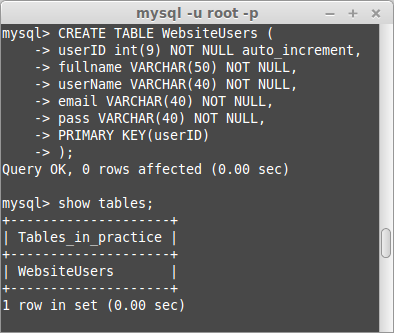
\includegraphics[width=.9\linewidth]{./pic/db.png}

\section{PHP routing}
\label{sec-2}
\begin{itemize}
\item tried to follow the tutorial from \url{https://www.youtube.com/watch?v=6reEBParHzQ}, but failed to make it work out within today's a few hours.
\item Good to have the debugging information showing up so that I have some clue what's going on. The reason it was failed last time turned out to be I didn't configure apache and enable mod$_{\text{rewrite}}$ module. Now problems are solved. References are pasted last part.
\end{itemize}

\section{Summary}
\label{sec-3}
\begin{itemize}
\item I had been mislead by course instructor's project deadline on "Course Work" which has listed to be 1/10/2016 11:55pm.
\item I noticed the course instructor changed the deadline for project due time through the 12/30/2015 announcement last night (this morning) around 1:00am.
\item When I download the final exam questionnaire form the website as study guide on 12/31/2015, I checked the "Coursework" project deadline is still 1/10/2016, so I have NOT check the website ever since that day.
\item I checked the website middle night in the early morning trying to see if there is any new material for the final exam, then noticed the announcement on 12/30/2015.
\item I am currently seeking place to move in, and got especially tired recent days (yesterday has staff on hands from 7:30am - today 1:30am)
\item When I learn this news, I am confident and believe I could finish my project successfully on time as the original due time, and that's reason when I have time and energy, I try to focus on something I am interested, rather than stick to some not so interested project.
\item But the confidence does NOT mean that I could successfully finish a project within a few hours, especially when I have got tired the day before already.
\item So I tried reach to the course instructor and get some extension. I wrote to him at 1:07am.
\item I worked sometime to get signup/login to some extent into shape, and then changed the topic to build PHP routing.
\item The linux LAMP for MySQL is pretty easy, but trying to understand and code the routing part took me quite some hours (due to headache), and has NOT solve this problem yet, but as usual, this does NOT affect my confidence at all. I believe in myself that with reasonable amount of time, I could solve the problem I am into.
\item Instead of any FAILURE, this experience rather warns me to pay attention to course instructor's deadline more carefully then beat/destroy any of my confidence.
\item I don't have any window's system, and the classmates know about this. I will try to reach the course instructor when I have chance to talk to him.
\item I may have misunderstood the 4 pages, cause once I linked the "SignUp/Login" button correctly, it includes FOUR page design already. Will double check with the advisor tonight.
\end{itemize}

\section{Requirements}
\label{sec-4}
\begin{itemize}
\item Use the  sample html and css file provided in the course resources folder to build a home page for your website.
\item You can customize the page by modifying html and css files. Use your own colors and images.
\item You will be creating a minimum of 4 pages or more website.
\item The subsequent pages should have the same header, left navigation and footer, but the body may contain different.
\item Provide a sign in /signup option in the landing page.
\item On page to add html forms and process the form data using php on the server.
\item Use javascript, angJavscript and PHP code where ever needed
\end{itemize}

\section{References}
\label{sec-5}
\begin{itemize}
\item Linux LAMP: \url{https://www.digitalocean.com/community/tutorials/how-to-install-linux-apache-mysql-php-lamp-stack-on-debian-8}
\item connecting MySQL: \url{https://help.ubuntu.com/community/ApacheMySQLPHP}
\item PHP signup: \url{http://mrbool.com/how-to-create-a-sign-up-form-registration-with-php-and-mysql/28675}
\item URL routing: \url{https://www.youtube.com/watch?v=6reEBParHzQ}
\item Apache configure: \url{http://blog.csdn.net/txl199106/article/details/40054939}
\item debugging options set: \url{http://stackoverflow.com/questions/17693391/500-internal-server-error-for-php-file-not-for-html}
\item Apache Load mod$_{\text{rewrite}}$: \url{http://roshanbh.com.np/2008/04/check-enable-mod_rewrite-apache.html}
\item enable apache mod$_{\text{rewrite}}$: \url{http://tecadmin.net/enable-apache-mod-rewrite-module-in-ubuntu-linuxmint/}\#
\item rewrite: \url{https://wordpress.org/support/topic/the-requested-url-wordpresscuriositywp-admin-was-not-found-on-this-server}
\item \url{https://wordpress.org/support/topic/the-requested-url-login-was-not-found-on-this-server-1}
\item mod$_{\text{rewrite}}$: \url{http://alexmansfield.com/linux/apache-mod_rewrite-in-ubuntumint}
\item mod$_{\text{rewrite}}$: \url{http://tecadmin.net/enable-apache-mod-rewrite-module-in-ubuntu-linuxmint/}
\item mod$_{\text{rewrite}}$: \url{http://xmodulo.com/how-to-enable-mod_rewrite-in-apache2-on-debian-ubuntu.html}
\end{itemize}
% Emacs 24.3.1 (Org mode 8.2.7c)
\end{document}